\documentclass[letterpaper]{article}
\usepackage[utf8]{inputenc}
\usepackage{enumerate}
\usepackage{xcolor}
\usepackage{graphicx}
\usepackage{multicol}
\usepackage{amsmath}
\usepackage{tabularx}
\usepackage{multirow}
\usepackage[spanish,es-nodecimaldot, es-tabla]{babel}
\usepackage{wrapfig}
\usepackage[rightcaption]{sidecap}
\graphicspath{ {./images/} }
\usepackage{amssymb}
\usepackage{setspace}
\usepackage{fancyhdr}
\usepackage[left=2.5 cm,right=2.5 cm, top=2.5 cm, bottom=2.5 cm]{geometry}
\usepackage{float}
\usepackage{afterpage}
\usepackage{tikz}
\usetikzlibrary{arrows.meta, decorations.pathreplacing}

% Configuración de encabezado y pie de página
\pagestyle{fancy}
\fancyhf{} % Limpia encabezado y pie
\fancyhead[R]{\small Estudiante de posgrado, Centro de Investigaciones en Óptica \\ Metrología Óptica}
\fancyfoot[C]{\thepage} % Número de página centrado
\renewcommand{\headrulewidth}{0pt} % Quita la línea bajo el encabezado
\renewcommand{\footrulewidth}{0pt} % Quita línea sobre pie de página

\begin{document}
	
	\begin{center}
		\Large \textbf{HOLOGRAFÍA DIGITAL: RECONSTRUCCIÓN MEDIANTE LA APROXIMACIÓN DE FRESNEL}
	\end{center}
	
	\begin{center}
		Jonathan Francisco Rojas Martínez\\
		jonathan.frm@cio.mx\\
		16/08/2026\\
		Centro de Investigaciones en Óptica\\
		Loma del Bosque 115, Lomas del Campestre, León, Gto, C.P. 37150
	\end{center}
	
	\begin{center}
		{\Large \textbf{Resumen}}
	\end{center}
	
	\noindent
	En esta práctica se implementó la técnica de holografía digital para registrar y reconstruir numéricamente el frente de onda óptico (amplitud y fase) de un objeto difusor bajo estudio. Se utilizó un montaje interferométrico con una fuente láser coherente y un sensor CCD para capturar el holograma digital. La reconstrucción computacional se llevó a cabo utilizando la aproximación de difracción de Fresnel, implementando la Transformada Discreta en un script de Python. Se logró obtener exitosamente tanto la imagen de intensidad como el mapa de fase directa del objeto, eludiendo el uso de revelados fotoquímicos y demostrando el potencial de la técnica para llevar a cabo metrología óptica de alta precisión a partir de una única imagen.
	
	\begin{multicols}{2}
		
		\section*{Introducción}
		
		La holografía digital representa un parteaguas en la ciencia óptica, ya que por primera vez es posible medir directamente la fase de una onda de luz utilizando tecnología electrónica de adquisición y computación. 
		
		El holograma, entendido como un patrón de interferencia microscópico originado por la superposición de un haz de referencia y un haz reflejado por el objeto, puede ser digitalizado a través de una cámara CCD. Sin embargo, para extraer la información útil y generar una imagen visible del objeto, se requiere de una reconstrucción digital.
		
		Dicha reconstrucción se aborda mediante métodos numéricos que simulan la propagación del frente de onda desde el plano del holograma hasta el plano de observación situado a una distancia $d$. Uno de los métodos más eficaces es la aproximación de difracción de Fresnel-Kirchhoff. Al asumir que la distancia de propagación es mayor a las distancias laterales e introduciendo una expansión de Taylor, la propagación de la luz puede interpretarse matemáticamente como una Transformada de Fourier multiplicada por una función de fase cuadrática (función Chirp).
		
		\section*{Objetivos}
		
		\begin{itemize}
			\item Comprender el fenómeno de interferencia y registro de hologramas para la extracción del campo electromagnético.
			\item Implementar la Transformada Discreta de Fresnel en lenguaje Python para reconstruir digitalmente tanto la intensidad como la fase de un objeto de prueba.
			\item Analizar experimentalmente el comportamiento numérico de la distancia de enfoque $d$ y los límites de resolución establecidos por el arreglo del sensor CCD.
		\end{itemize}
		
		\section*{Material y equipo}
		
		\begin{enumerate}
			\item Láser de estado sólido (e.g., Nd:YAG a 532 nm)
			\item Cámara CCD monocromática
			\item 2 Divisores de haz (Beam splitters)
			\item Objetivo de microscopio x20
			\item 2 Fibras ópticas
			\item 2 dados de diferentes tamaños
			\item Monturas mecánicas
			\item PC con cámara CCD y programa de captura de imágenes.
		\end{enumerate}
		
		\section*{Procedimiento}
		
		\begin{enumerate}[i)]
			\item Divida el haz con el cubo divisor en dos, acople los haces a las fibras ópticas y seleccione uno como el haz objeto y el otro como haz de referencia.
			\item Superponga el haz de referencia sobre el detector CCD, asegurando que el ángulo de incidencia respecto al haz objeto cumpla estrictamente con el criterio de Nyquist para prevenir \textit{aliasing}.
			\item Adquiera y guarde la imagen del patrón de interferencia (Holograma digital).
			\item Desarrolle un programa en Python que cargue el arreglo matricial de la imagen. Incorpore los parámetros del tamaño del píxel ($\Delta\xi, \Delta\eta$) y la longitud de onda ($\lambda$).
			\item Aplique la aproximación de Fresnel: multiplique computacionalmente el holograma por la onda de referencia conjugada digital y por el factor exponencial cuadrático.
			\item Ejecute una Transformada Rápida de Fourier (FFT) bidimensional para obtener la distribución del campo complejo en el plano de reconstrucción.
			\item Programe el software para poder iterar o ajustar el valor numérico de la distancia $d$ hasta encontrar el enfoque nítido de la imagen de intensidad. Extraiga y visualice tanto el módulo como la fase del frente de onda reconstruido.
		\end{enumerate}
		
		\section*{Resultados y Análisis}
		
		Para la recuperación de la información compleja se debieron calibrar los parámetros de captura físicos contra los valores lógicos del algoritmo de Python.
		
		\begin{table}[H]
			\centering
			\caption{Parámetros del Sistema y Reconstrucción}
			\vspace{0.3cm}
			\resizebox{\columnwidth}{!}{%
				\begin{tabular}{|m{2.5cm}|m{2.2cm}|m{3.2cm}|}
					\hline
					\multicolumn{3}{|c|}{\textbf{Variables de Fresnel Discreto}} \\
					\hline
					\centering \textbf{Parámetro} & \centering \textbf{Valor} & \centering \textbf{Descripción} \arraybackslash \\
					\hline
					Longitud de onda ($\lambda$) & 532 nm & Emisión del láser Nd:YAG empleado. \\ \hline
					Distancia ($d$) & 20 cm y 11.5 cm& Distancia numéricamente ajustada para enfocar. \\ \hline
					Muestreo ($\Delta\xi \times \Delta\eta$) & 6.45 $\mu$m $\times$ 6.45 $\mu$m & Tamaño de píxel físico de la CCD. \\ \hline
				\end{tabular}%
			}
		\end{table}
		
		\vspace{0.3cm}
		
		La adquisición generó un patrón altamente denso de speckel, producto de la naturaleza aleatoria del objeto difuso y la portadora espacial introducida por el haz de referencia.
		s
		
		Al someter la imagen a la propagación numérica descrita en la Ecuación central de la aproximación de Fresnel, se obtuvo la distribución espectral de intensidad y fase. La imagen exhibe la amplitud del campo logrando reproducir detalles del objeto. (Las imágenes están al final del documento)
		
		
		
		\section*{Cuestionario}
		\begin{enumerate}
			\item \textbf{Explique por qué, matemáticamente, no se puede simplemente aproximar a $z$ el término $r$ en el exponente de la función de propagación de Huygens.}\\
			Aunque $z$ (la distancia longitudinal) es mucho mayor que las coordenadas transversales, la distancia $r$ en el término de fase exponencial ($e^{-ikr}$) está multiplicada por el número de onda $k = 2\pi/\lambda$. Al ser $\lambda$ del orden de nanómetros, un error minúsculo en la aproximación de $r$ causaría un desplazamiento masivo en múltiplos de $2\pi$ para la fase de la onda. Por ello, es imperativo mantener los términos cuadráticos de la expansión de Taylor.
			
			\item \textbf{¿Qué implicación experimental tiene el tamaño del píxel del detector CCD ($\Delta\xi$) según el Teorema de Nyquist?}\\
			El CCD es un medio de muestreo discreto. Para que el holograma grabe correctamente las altas frecuencias espaciales producidas por la interferencia, la distancia física entre franjas debe ser cubierta por al menos dos píxeles ($s > 2\Delta\xi$). Esto condiciona el experimento restringiendo el ángulo máximo permisible entre el objeto y la referencia, dictando también el ancho máximo del objeto ($d_0$) que el sistema puede capturar a cierta distancia.
			
			\item \textbf{¿Qué ocurre numéricamente si introducimos una distancia de propagación $d$ errónea en nuestro script de reconstrucción?}\\
			El término exponencial cuadrático (función Chirp) actuará con una curvatura incorrecta. Esto ocasiona que las ondas esféricas simuladas no coincidan en el plano imagen real del objeto, provocando que la imagen de intensidad reconstruida aparezca borrosa y completamente desenfocada, emulando físicamente a una cámara fuera de foco.
		\end{enumerate}
		
		\section*{Conclusiones}
		La práctica confirmó la validez de la aproximación discreta de Fresnel como una herramienta de alto impacto en la holografía digital para la extracción matemática del campo complejo. A diferencia del revelado fotoquímico histórico, el entorno computacional facilitó no solo visualizar la amplitud del campo electromagnético en un monitor, sino también decodificar la fase óptica. Se comprobó la sensibilidad del montaje respecto al teorema de muestreo, requiriendo un ajuste meticuloso del ángulo entre los brazos interferométricos para evitar exceder las frecuencias de corte dictadas por los pixeles de $5.2\,\mu\text{m}$. La flexibilidad del algoritmo de Python, que emula la propagación de onda en el espacio libre variando un único parámetro $d$, subraya la versatilidad de la metrología óptica digital moderna para estudios de micro-topografía, ensayos no destructivos y dinámica de materiales.
		
		\section*{Bibliografía}
		\begin{enumerate}
			\item U. Schnars, C. Falldorf, \textit{Digital Holography and Wavefront Sensing}. Springer.
			\item J. W. Goodman, \textit{Introduction to Fourier Optics}. Roberts \& Co.
			\item T. Kreis, \textit{Handbook of Holographic Interferometry}. Wiley-Vch.
		\end{enumerate}
		
	\end{multicols}
	
	\begin{figure}[H]
		\centering
		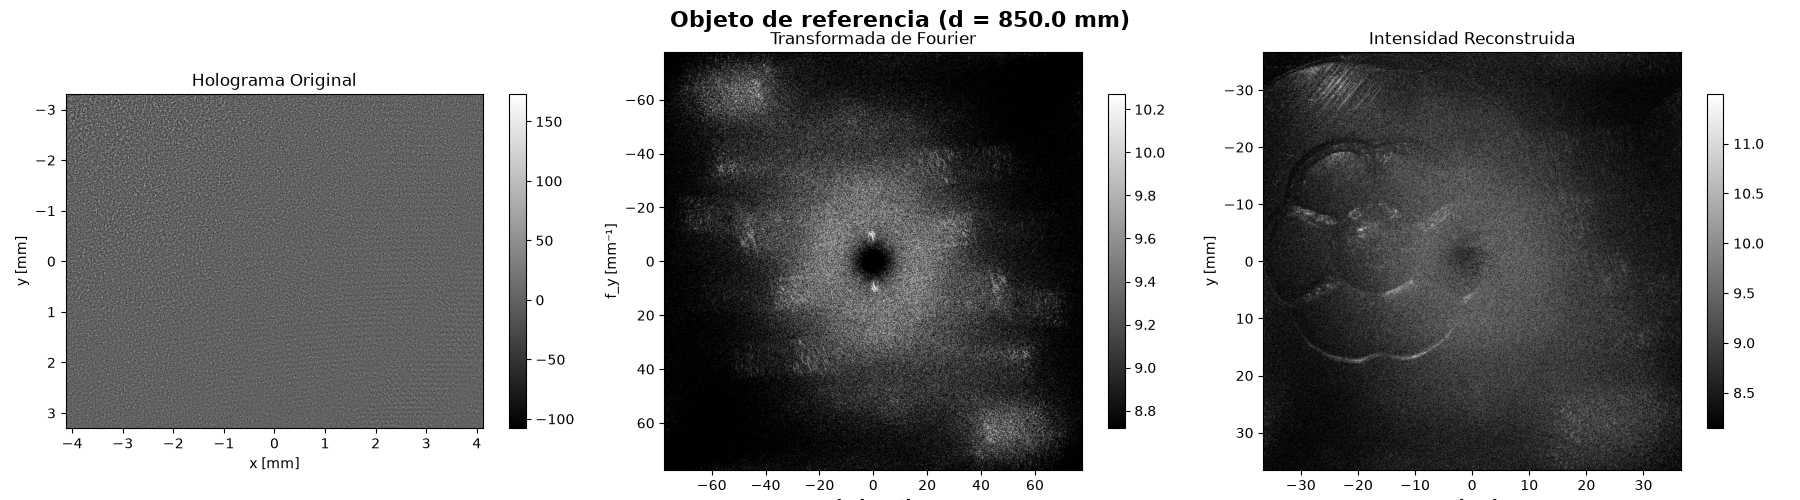
\includegraphics[width=\linewidth]{ob_ref.png}
		\caption{Objeto de referencia.}
		\label{fig:fase}
	\end{figure}

\begin{figure}[H]
	\centering
	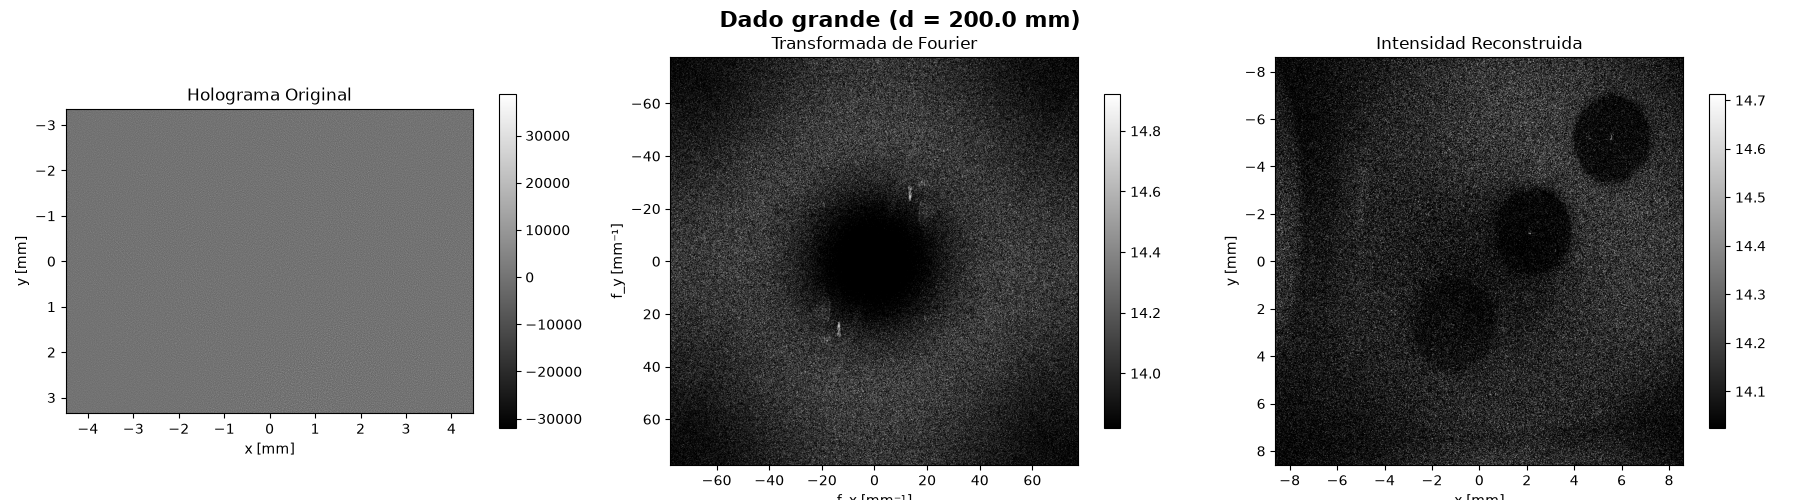
\includegraphics[width=\linewidth]{dado_pequeno.png}
	\caption{Dado grande.}
	\label{fig:fase}
\end{figure}

\begin{figure}[H]
	\centering
	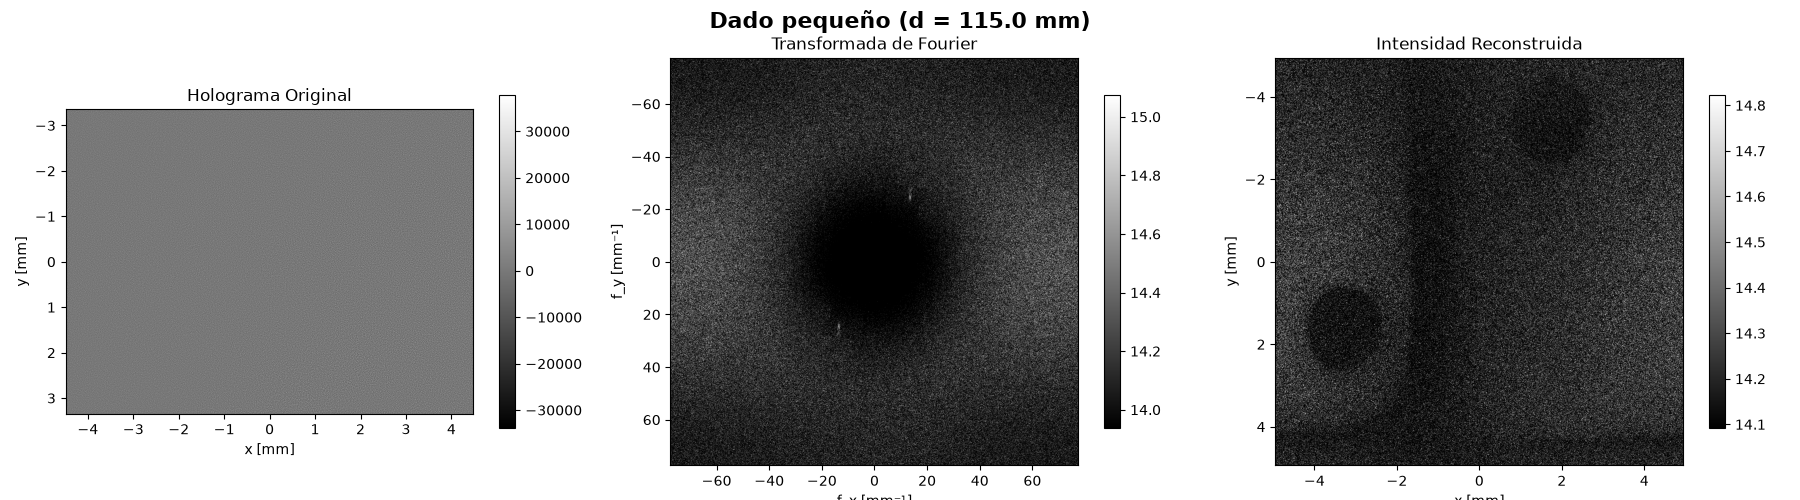
\includegraphics[width=\linewidth]{dado_grande.png}
	\caption{Dado pequeño.}
	\label{fig:fase}
\end{figure}


	
\end{document}
